\documentclass{article}
\usepackage{xeCJK}

\usepackage[english]{babel}
\usepackage{listings}
\usepackage{minted}

\usepackage[letterpaper,top=2cm,bottom=2cm,left=3cm,right=3cm,marginparwidth=1.75cm]{geometry}

% Useful packages
\usepackage{ragged2e}
\usepackage{amsmath}
\usepackage{comment}
\usepackage{graphicx}
\usepackage{IEEEtrantools}
\usepackage[hyphens]{url}
\usepackage[colorlinks=true, allcolors=blue]{hyperref}

\title{Aptos 区块链:安全、可扩展和可升级的 Web3 基础设施}
\author{}
\date{2022年 8月 11日\\v1.0 中文版 \footnote{特别鸣谢此白皮书的\href{https://github.com/move-dao}{MoveDao}翻译人员:\href{https://github.com/halfswing}{Boyu}, \href{https://github.com/ruy1su}{Ruyisu},\href{https://github.com/lshoo}{lshoo},\href{https://github.com/Container-00}{Container}, \href{https://github.com/Kusou1}{Kusou1}, ywww,肖川, Tom, \href{https://github.com/geometryolife}{JoeChen}(排名不分先后)}}

\begin{document}
\maketitle

\begin{abstract}
{区块链是一种新的互联网基础设施,随着区块链的兴起,开发人员以快速增长的速度部署了数以万计的去中⼼化应⽤程序。不幸的是,由于频繁中断、高成本、低吞吐量限制和众多安全问题,区块链的使用尚未普及。为了在web3时代实现大规模应用,区块链基础设施需要借鉴云基础设施的路径,成为构建⼴泛使⽤的应⽤程序的可信、可扩展、具有成本效益且不断改进的平台。  

我们展⽰了以可扩展性、安全性、可靠性和可升级性为关键原则设计的 \emph{Aptos} 区块链,用以应对这些挑战。Aptos区块链在过去三年中由全球超过 350 名开发⼈员设计开发\cite{aptos_core_github}。它在共识、智能合约设计、系统安全、性能和去中⼼化⽅⾯提供了新的创新。这些技术的结合将为web3推向⼤众提供⼀个基本的构建块:\footnote{法律免责声明:本白皮书及其内容不是任何代币的出售要约或购买要约的邀请。我们发布此白皮书仅是为了接收公众的反馈和意见。本文档中的任何内容均不应被阅读或解释为Aptos 区块链或其代币(如果有)将如何开发、使用或增值的保证或承诺。 Aptos 仅概述了其当前的计划,这些计划可能会自行改变,其成功将取决于其无法控制的许多因素。此类未来陈述必然涉及已知和未知的风险,这可能导致未来期间的实际表现和结果与我们在本白皮书中描述或暗示的内容存在重大差异。 Aptos 不承担更新其计划的义务。无法保证白皮书中的任何陈述将被证明是准确的,因为实际结果和未来事件可能存在重大差异。请不要过分依赖未来的陈述。}
}

\begin{itemize}
 \item 第一,Aptos区块链在本地集成并在内部使用\emph{Move语言},以实现快速安全的交易执行\cite{move_github}。此外,我们还提供了名为\emph{Move prover}的智能合约形式化验证器,由此为Move合约的不变性和行为提供额外的保障。这种对安全性的关注使得开发人员能够更好地保护他们的软件免受恶意实体的侵害。

 \item 第二,Aptos数据模型支持灵活的密钥管理和混合托管选项。这与签名前的交易透明度和实用的轻型客户端协议一起,提供了更安全、更可信的用户体验。  

 \item 第三,为了实现高吞吐量和低延迟,Aptos 区块链在交易处理的关键阶段采⽤了流⽔线和模块化⽅法。具体来说,交易传播、区块元数据排序、并行交易执行、批量存储和账本认证都是同时运行的。这种方法充分利用了所有可用的物理资源,提高了硬件效率,并实现了高度并行执行。

 \item 第四,与其他通过要求预先了解数据读写来打破事务原子性的并行执行引擎不同,Aptos 区块链不会对开发⼈员施加此类限制。它可以有效地⽀持任意复杂事务的原⼦性,从而为现实世界的应⽤程序实现更⾼的吞吐量和更低的延迟,并简化开发。 

 \item 第五,Aptos 模块化架构设计⽀持客户端灵活性,并针对频繁和即时升级进行了优化。此外,为了快速部署新技术创新并⽀持新的 web3 ⽤例,Aptos 区块链提供了嵌⼊式链上变更管理协议。 

 \item 最后,为了超越单个验证器的性能,Aptos区块链正在试验前卫的举措:其模块化设计和并行执行引擎支持验证器内部分片,同质状态分片提供了水平吞吐量可扩展性的潜力,而不会增加节点运营商的额外复杂性。

\end{itemize}

\end{abstract}

\section{介绍}

在互联⽹的 web2 版本中,消息传递、社交媒体、⾦融、游戏、购物和⾳频/视频流等服务由控制⽤户数据直接访问的中⼼化公司提供(例如,Google、Amazon、Apple、和Meta)。这些公司使⽤针对⽬标⽤例优化的特定应⽤软件开发基础架构,并利⽤云基础设施向用户部署这些应用程序。云基础设施提供对虚拟化或者物理基础设施服务的访问,例如租⽤的虚拟机 (VM) 和在全球数据中⼼(例如 AWS、Azure 和 Google Cloud)内运行的裸机硬件。因此,构建可扩展到数⼗亿⽤户的 web2 互联网服务从未像今天这样容易。 然⽽,web2 要求⽤户明确信任中⼼化实体,这⼀要求让社会越来越担忧。

为了消除这种担忧,⼀个新的互联⽹时代已经开始:web3。在互联⽹的 web3 版本中,\emph{区块链}已经出现,其提供了去中心化、不可变的账本,使⽤户能够安全可靠地相互交互,而无需信任任何控制中介或中⼼化实体。类似于 web2 互联⽹服务和应⽤程序如何依赖云基础设施作为构建块,去中⼼化应⽤程序可以使⽤区块链作为去中⼼化基础设施层,从而覆盖全球数⼗亿⽤户。

然⽽,尽管当今存在许多区块链,但web3尚未被广泛应用 \cite{a16_state}。虽然技术不断推动行业发展,但现有区块链不可靠,对⽤户收取⾼额交易费⽤,吞吐量受限,因安全问题经常遭受资产损失,并且⽆法⽀持实时响应。与云基础设施如何使 web2 服务达到数⼗亿相⽐,区块链尚未使 web3 应⽤程序达到相同的效果。


\section{Aptos的愿景}

Aptos 的愿景是提供⼀个区块链,可以为 web3 带来主流应⽤,并增强去中⼼化应⽤程序的⽣态系统,以解决现实世界的⽤户问题。我们的使命是通过提供灵活的模块化区块链架构来提升区块链可靠性、安全性和性能⽅⾯的最新技术⽔平。该体系架构应⽀持频繁升级、 快速采⽤最新技术进步,以及对新兴⽤例提供⼀流的⽀持。

我们设想⼀个使⽤它进行社区管理和运营的去中⼼化、安全和可扩展的⽹络。当全球基础设施需求增长时,区块链的计算资源会横向和纵向扩展以满⾜这些需求。随着新⽤例和技术进步的出现,⽹络应该在不中断⽤户的情况下频繁且⽆缝地升级。对基础设施的担忧应该逐渐消失。开发⼈员和⽤户将可以访问许多不同的选项,⽤于密钥恢复、数据建模、智能合约标准、资源使⽤权衡、隐私和可组合性。⽤户知道他们的资产是安全的、始终可⽤的,并且可以以接近成本的费⽤进行访问。任何⼈都可以安全、轻松、不变地与全球不受信任的各⽅进行交易。区块链与云基础设施⼀样⽆处不在。 

为了实现这⼀愿景,必须取得重⼤的技术进步。我们在过去三年中构建、开发、推进和部署 Diem 区块链(Aptos 区块链的前⾝)的经验证明,⽹络可以在不中断其客户端的情况下不断升级其协议\cite{diem_blockchain}。 2020 年初,Diem 主⽹部署到⼗几家节点运营商,拥有多个钱包提供商。在接下来的⼀年里,我们的团队发布了两次重⼤升级,改变了共识协议和核⼼框架。两次升级都在⽤户没有停机的情况下完成。在 Aptos 区块链上,我们对技术堆栈进行了⼀系列彻底的改进,同时还将安全、透明和频繁的升级作为核⼼功能,这是受到了Diem区块链的启发。特别是,我们强调了交易处理的新⽅法(如第 \ref{sec:pipelining_batching} 节所述)以及去中⼼化和⽹络治理的新⽅法。

随着 Aptos 区块链的不断改进和发展,我们将发布本⽩⽪书的更新版本,其中包含我们协议和设计选择的最新迭代。在本⽂档的其余部分,我们将描述 Aptos 区块链的当前状态以及未来计划。 

\begin{figure}
\centering
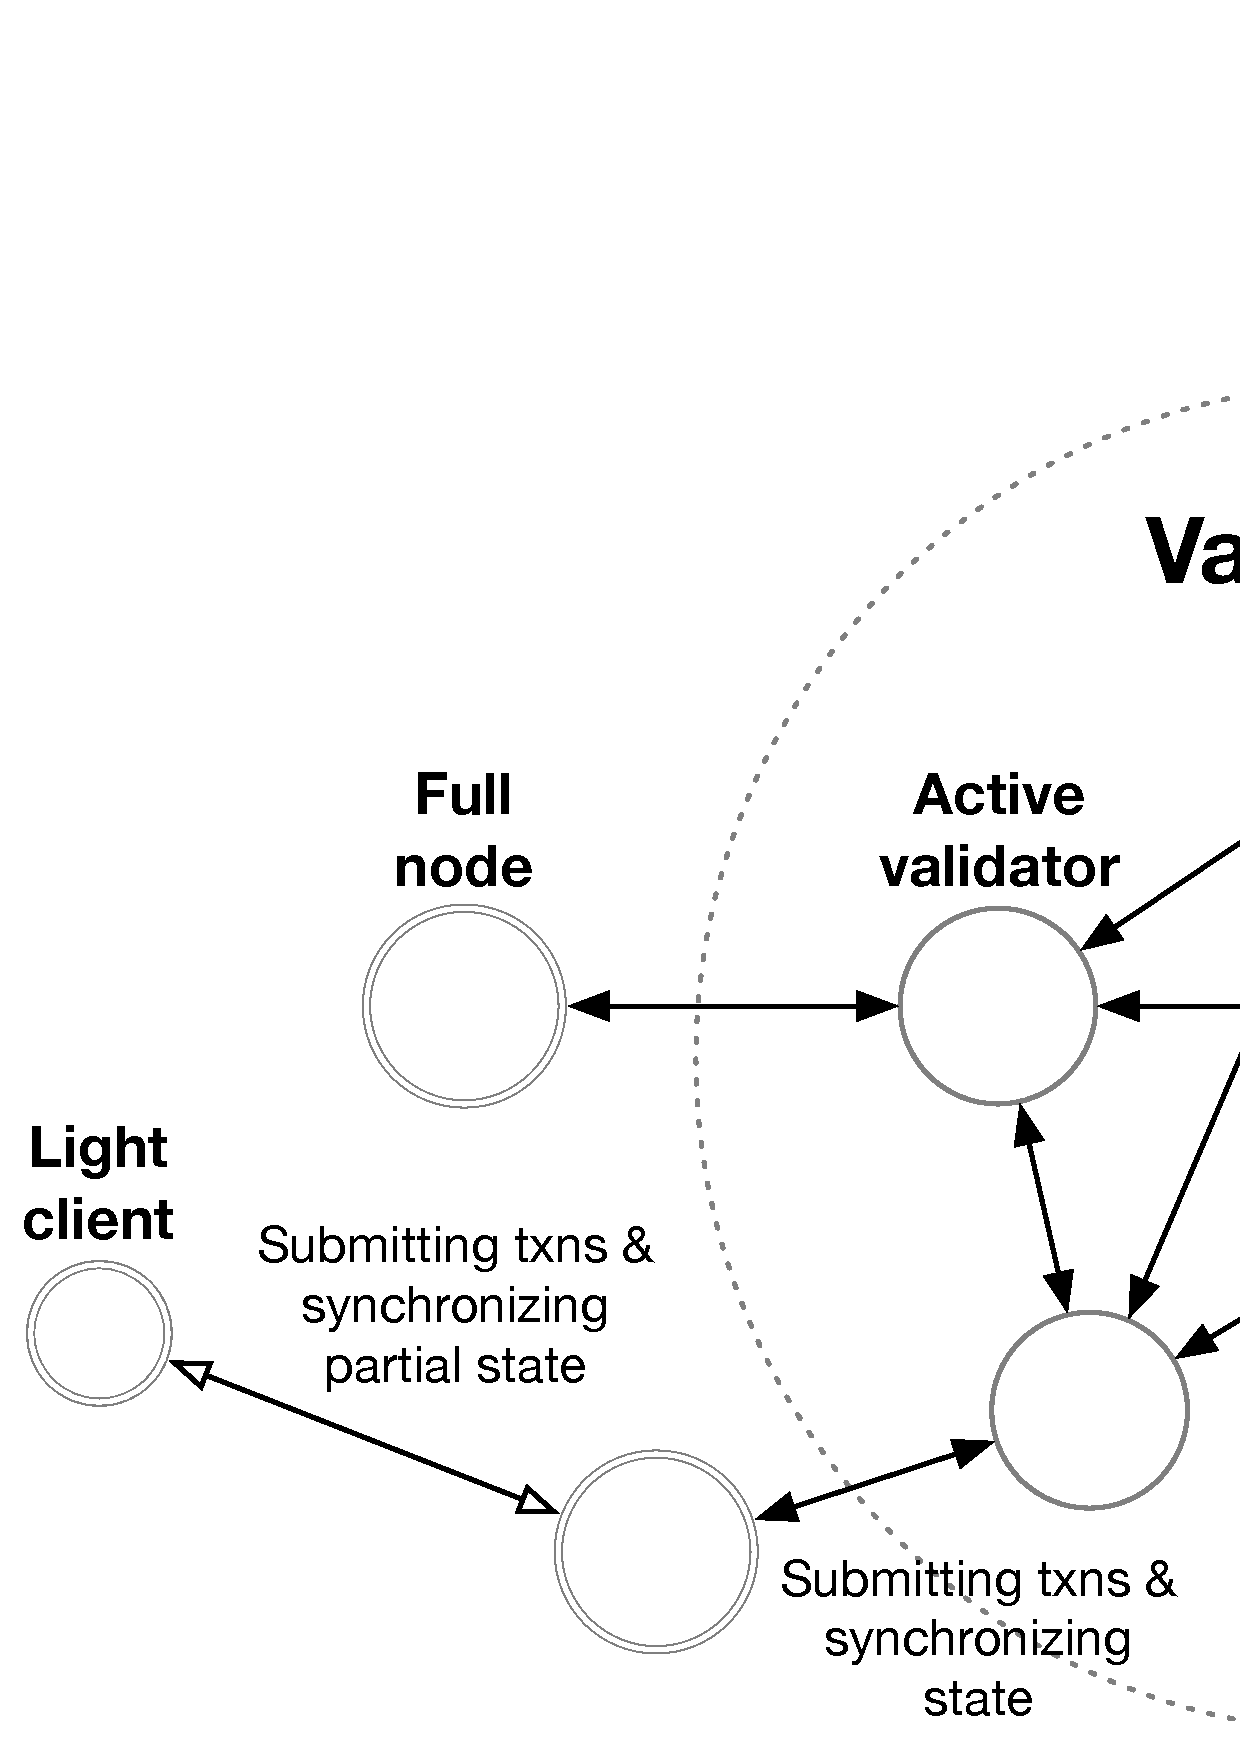
\includegraphics[width=0.95\textwidth]{validators.png}
\caption{\label{fig:aptos_ecosystem}Aptos 生态的组成部分。}
\end{figure}

\section{概述}

如图 \ref{fig:aptos_ecosystem} 所⽰,Aptos 区块链由⼀组\emph{验证者节点}组成,它们使⽤拜占庭容错 (\emph{BFT})、权益证明共识机制(POS)共同接收和处理来⾃⽤户的交易。代币持有者在其选定的验证者节点中锁定或\emph{质押}代币。每个验证者节点的共识投票权重与质押其中的数量成正⽐。验证者节点可以是\emph{活跃的}并参与共识。同样,如果验证者节点没有⾜够的权益参与、轮换出验证者节点集合、选举(类似同步区块链状态)时离线,或者由于历史性能不佳⽽被共识协议视为不参与,验证器也可能处于\emph{⾮活动状态}。 

\emph{客户端}是所有需要接受系统提交交易或查询区块链状态和历史的入口部分。客户可以选择下载并验证由验证者节点签名的查询数据证明。\emph{全节点}是从验证者节点或⽹络中的其他全节点复制交易和区块链状态的客户端。他们可以根据需要选择修剪交易历史和区块链状态以回收存储。\emph{轻客户端}仅维护当前的一组验证器,并且可以安全地查询部分区块链状态,通常是来⾃完整节点。钱包是轻客户端的常见⽰例。

为了满⾜⼴泛采⽤安全、快速、可靠和可升级的 web3 基础架构的需求,Aptos 区块链建⽴在以下核⼼设计原则之上:

\begin{itemize}
\item 通过一种新的智能合约编程语⾔Move \cite{move},快速安全地执行,具有简单的可审计性和静态分析性。 Move 起源于 Aptos 区块链的前⾝,并随着该项⽬的发展⽽不断进步。 

\item 通过批处理、流水线和并行化的事务处理方法,实现极高的吞吐量和低延迟。

\item 新颖的并行事务处理,通过Block-STM 有效地⽀持任意复杂事务的原⼦性,这与需要预先了解要读取和写⼊的数据位置的现有并行执行引擎不同。

\item 通过快速的权益权重验证者节点集合和声誉跟踪实现性能优化以及去中心化。

\item 将可升级性和可配置性作为⼀流的设计原则,以拥抱新⽤例和最新技术。

\item 模块化设计支持严格的组件级测试,以及适当的威胁建模和无缝部署,所有这些都确保了⾼度安全和可靠的操作。 

\item 吞吐量可水平扩展,同时保持去中心化,其中分⽚是向⽤户公开的一等公民,也是编程和数据模型的原⽣概念。
\end{itemize}

第 \ref{sec:move} 节解释了开发⼈员如何与 Aptos 区块链中与 Move 交互。第 \ref{sec:logical} 节描述了逻辑数据模型。第 \ref{sec:user} 节详细介绍了 Aptos 区块链如何通过强⼤的验证⽅法实现安全的⽤户体验。第 \ref{sec:pipelining_batching} 节描述了围绕流⽔线、批处理和并行化的关键性能创新。第 \ref{sub:state_sync} 节详细介绍了不同客户端与其他节点同步状态的各种选项。第 \ref{sec:community_ownership} 节描述了我们的社区所有权和治理计划。最后,第 \ref{sec:performance} 节讨论了未来在保持去中⼼化的同时性能优化的⽅向。


\section{Move 语言}
\label{sec:move}

Move 是⼀种新的智能合约编程语⾔,强调安全性和灵活性。 Aptos 区块链使⽤ Move 的对象模型来表⽰其账本状态(参见第 \ref{sub:ledger_state} 节) ,并使⽤ Move 代码(模块)对状态转换规则进行编码。⽤户提交的交易可以发布新模块、升级现有模块、执行模块内定义的入口函数,或者包含可以直接与模块公共接⼝交互的脚本。

Move ⽣态系统包含编译器、虚拟机和许多其他开发⼯具。 Move 受到 Rust 编程语⾔的启发,该语言通过线性类型等概念明确了数据的所有权。 Move强调资源稀缺性、保护性和访问控制。Move模块定义了每个资源的⽣命周期、存储和访问模式。这确保了像 \mintinline{rust}{Coin} 这样的资源不会在没有适当凭证的情况下产⽣,不会被双花,也不会消失。

即使存在不受信任的代码,Move 也利⽤字节码形式化验证来保证类型和内存安全。为了帮助编写更受信任的代码,Move 包含了⼀ 个正式的形式化验证器,即 Move Prover \cite{move_prover},它能够根据给定规范验证 Move 程序的功能正确性,该规范是用集成到 Move 中的规范语⾔制定的。 

除了⽤户账户和相应的账户内容外,账本状态还包含 Aptos 区块链的链上配置。此⽹络配置包括⼀组活跃的验证节点、质押属性以及 Aptos 区块链中各种服务配置。Move 对模块可升级性和全⾯可编程性的⽀持实现了⽆缝变更配置,并⽀持对Aptos 区块链本⾝的升级(两组升级已多次执行,且在私有主⽹上实现零停机时间)。

Aptos 团队进⼀步增强了 Move,⽀持更⼴泛的 web3 ⽤例。如后⾯5.5节所述,Aptos 区块链支持细粒度资源控制。这不仅⽀持执行的并行化,⽽且还实现了与访问和修改数据相关的近乎固定的成本。此外,Aptos 区块链提供了建⽴在细粒度存储之上 Table ⽀持,允许在单个帐户中存储⼤规模数据集(例如,⼤量 的NFT 集合)。此外,Aptos ⽀持完全在链上表⽰的共享或⾃治帐户。这允许复杂的去中⼼化⾃治组织 (DAO) 协作共享帐户,并将这些帐户⽤作异构资源集合的容器。


\section{逻辑数据模型}
\label{sec:logical}

Aptos 区块链的\emph{账本状态}包含了所有账户的状态。账本状态使用一个 64 位无符号整数进行版本控制,该整数对应于系统已执行的交易数量。任何人都可以向 Aptos 区块链提交交易以修改账本状态。在执行交易时,会生成\emph{交易结果}。交易结果包含修改账本状态的零个或多个操作(称为\emph{写入集})、结果事件数组(vector)(参见第 \ref{subsub:events} 节)、消耗的gas量和交易的执行状态。

\subsection{交易(Transaction)}

已签名的交易包含以下信息: 

\begin{itemize}
\item \textbf{交易验证器}:发起人使用包含一个或多个数字签名的交易验证器来确保交易是否经过验证。 

\item \textbf{发起人地址}:发起人的帐户地址。 

\item \textbf{负载}:负载要么指链上现有的入口函数,要么包含要作为内联字节码(称为脚本)执行的函数。此外,一组输入参数被编码为字节数组。对于点对点交易,输入包含收件人的信息和转移给他们的金额。 

\item \textbf{Gas 价格}(指定的货币/Gas单位表示):这是发送方愿意为执行交易而为每单位 Gas 支付的金额。 Gas 是一种支付计算、网络和存储费用的方式。gas单位是计算的抽象度量,没有内在的现实世界价值。 

\item \textbf{最大 gas 量}:最大 gas 量是交易在中止之前允许消耗的最大gas 单位。账户必须至少有 gas 价格乘以最大 gas 量, 否则交易将在验证期间被丢弃。 

\item \textbf{序列号}:交易的序列号。这必须与交易执行时存储在发件人帐户中的序列号匹配。成功执行交易后,帐户序列号会增加以防止重放攻击。 

\item \textbf{过期时间}:一个时间戳,交易有效的截止时间。 

\item \textbf{链ID} : 标识此交易有效的区块链,提供进一步保护以防止用户防止签名错误。
\end{itemize}

在每个版本 $i$,状态变化由元组 $(T_i, O_i, S_i)$ 表示,分别包含交易、交易输出和结果账本状态。给定一个确定性函数 $\textsf{Apply}$,执行具有账本状态 $S_{i-1}$ 的交易 $T_i$ 会产生事务输出 $O_i$ 和一个新的账本状态 $S_i$。即,$\textsf{Apply}(S_{i-1}, T_i) \rightarrow \langle O_i, S_i\rangle$。

\subsubsection{事件}
\label{subsub:events}

在交易执行期间发出事件。每个 Move 模块都可以定义自己的事件并选择在执行时何时发出这些事件。例如,在Coin转移过程中,发送者和接收者的账户都会分别发出 \emph{SentEvent} 和 \emph{ReceivedEvent}。这些数据存储在账本中,可以通过 Aptos 节点进行查询。每个注册的事件都有一个唯一的键,该键可用于查询事件详情。 

向同一事件键发出的多个事件会产生\emph{事件流},这是一个事件列表,每个条目都包含一个从0开始依次增加的数字、一个类型和数据。每个事件必须由某种类型来定义。可能有多个事件由相同或相似的类型定义,特别是在使用泛型时。事件有相关的数据。对于Move模块的开发者来说,一般的原则是包括所有必要的数据,以了解在执行改变数据和发出事件的事务之前和之后对基础资源的变化。

交易只能生成事件,不能读取事件。这种设计允许交易执行仅是当前状态和交易输入(参数)的一个函数,而不是历史信息 (例如,以前产生的事件)。

\subsection{账户}
\label{sec:accounts}

每个帐户都由一个唯一的 256 位值识别,称为帐户地址。当一个从现有账户发送的交易调用 \mintinline{rust}{create_account(addr)} Move 函数时,会在账本状态下创建一个新账户(参见第 \ref{sub:ledger_state} 节)。 这通常发生在交易尝试将 Aptos 代币发送到尚未创建的帐户地址时。为方便起见,Aptos 还支持 \mintinline{rust}transfer(from, to, amount) 函数在收件人账户不存在的时候会隐式为其创建一个账户。

要创建一个新帐户,用户首先生成一个签名密钥对:$(vk, sk)$。接下来,使用与签名方案标识符 ($(ssid)$) 连接的公共验证密钥 $vk$ 的加密哈希 $H$ 推导出给定签名方案的新帐户地址:其中 $addr = H(vk, ssid)$。 

在地址 \mintinline{rust}{addr} 创建新帐户后,用户可以使用私有签名密钥 $sk$ 对要从 \mintinline{rust}{addr} 帐户发送的交易进行签名。用户还可以轮换 $sk$,以主动更改 $sk$ 或对可能的泄漏威胁作出反应。这不会更改帐户地址,因为创建时,从公共验证密钥。 

Aptos 区块链不会将账户与真实世界的身份相关联。用户可以通过生成多个密钥对来创建多个帐户。由同一用户控制的帐户彼此之间没有内在联系。但是,单个用户仍然可以在单个钱包中管理多个帐户,以进行简单的资产管理。这种灵活性为用户提供了匿名性,同时我们为未来的版本试验了保护隐私的基础。单个用户或一组用户拥有的多个帐户也提供了增加并发执行的通道,如第 \ref{subsec:parallel_transaction_execution} 节所述。

\begin{figure}
\centering
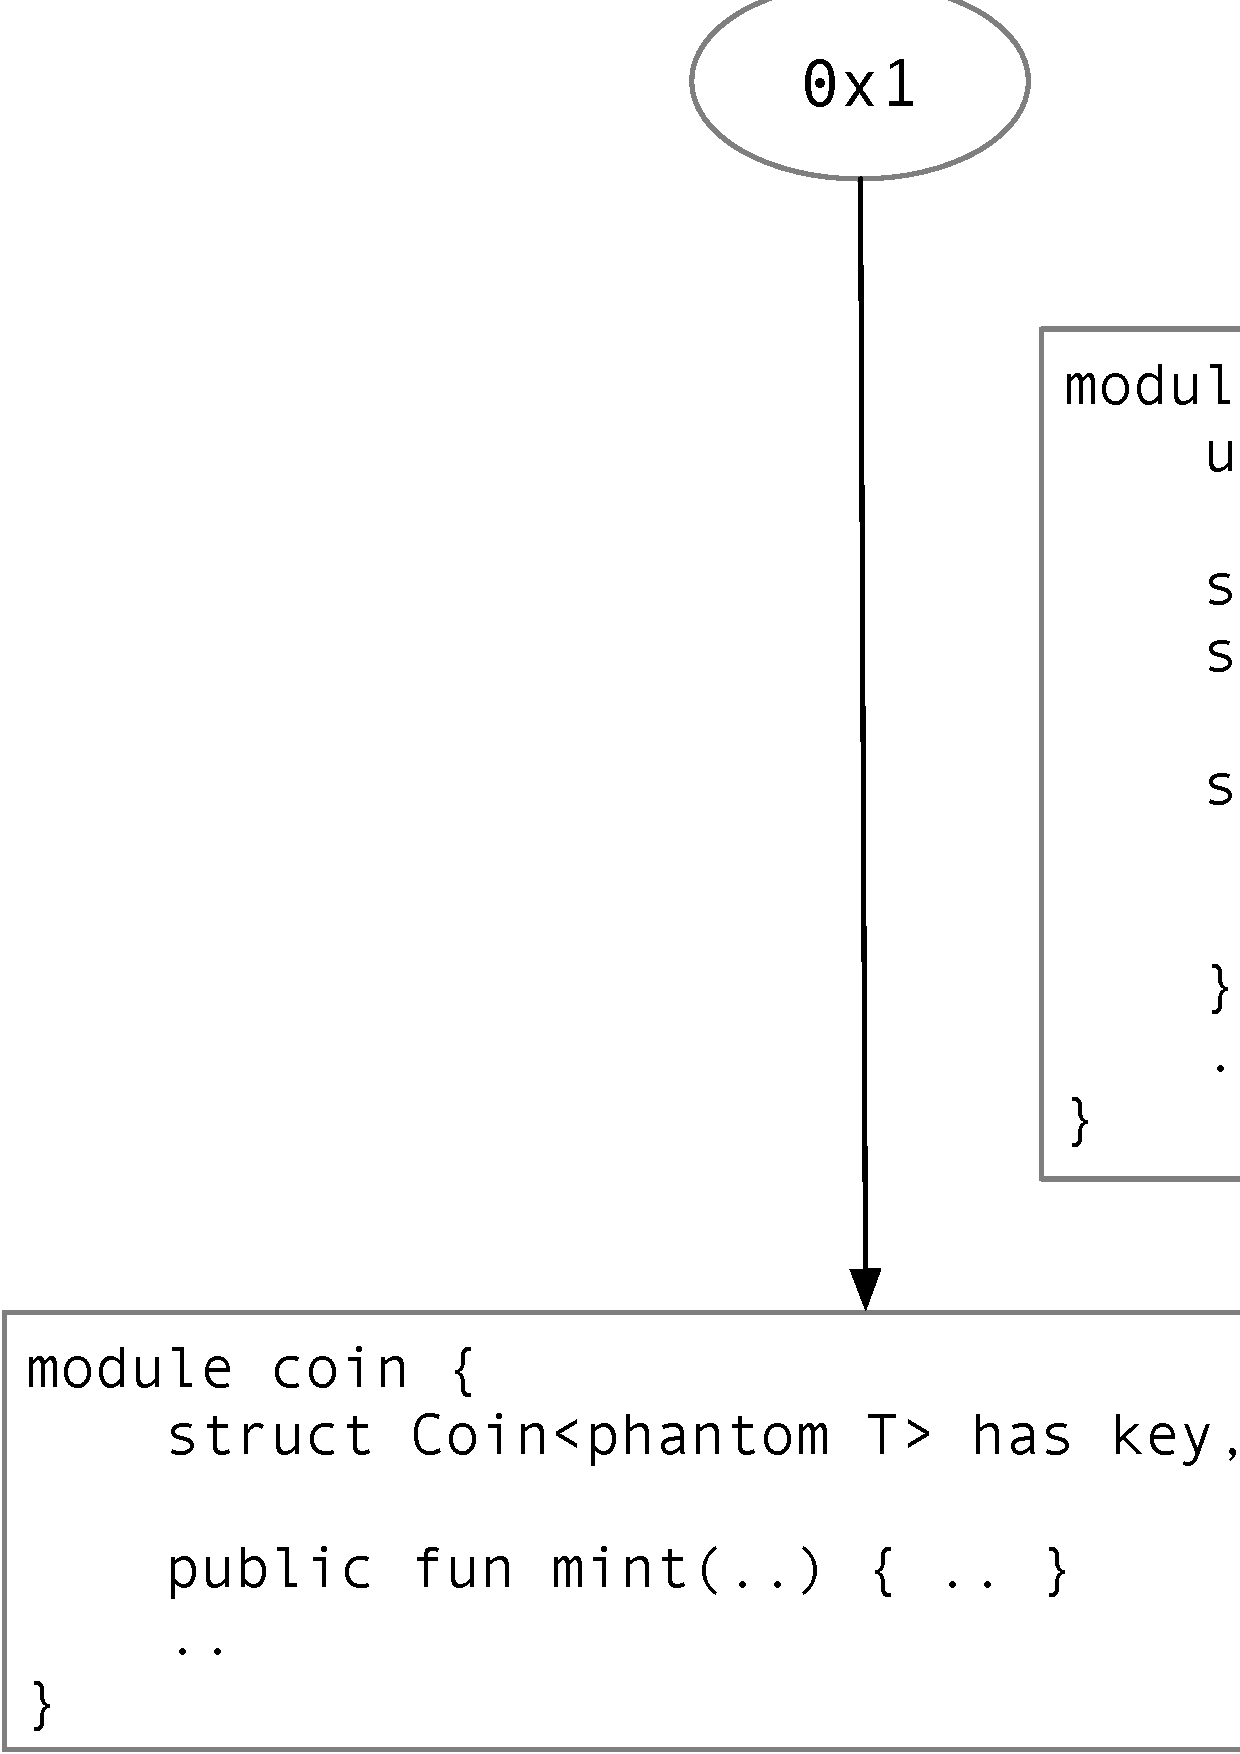
\includegraphics[width=0.95\textwidth]{move_1.png}
\caption{\label{fig:move_modules}链上的Move模块示例。}
\end{figure}

\subsection{Move 模块}
Move 模块包含声明数据类型(结构)和程序的 Move 字节码。它由声明模块的帐户地址和模块名称来标识。例如,图 \ref{fig:move_modules} 中第一个货币模块的标识符是\mintinline{rust}{0x1::coin}。一个模块可以依赖链上其他模块,如图 \ref{fig:move_modules} 中的 wallet 模块所示,从而实现代码重用。

一个模块在一个帐户中的命名必须是唯一的,即每个帐户最多可以声明一个具有任何给定名称的模块。例如,图 \ref{fig:move_modules}  中地址 0x1 的帐户无法声明另一个名为 \mintinline{rust}{coin} 的模块。另一方面,地址为 address \mintinline{rust}{0x3} 的账户可以声明一个名为 \mintinline{rust}{coin} 的模块,该模块的标识符为 \mintinline{rust}{0x3::coin}。请注意,\mintinline{rust}{0x1::coin::Coin} 和 \mintinline{rust}{0x3::coin::Coin} 是不同的类型,不能互换使用,也不能共享公共模块代码。相比之下,\mintinline{rust}{0x1::coin::Coin<0x2::wallet::USD>} 和 \mintinline{rust}{0x1::coin::Coin<0x2::wallet::JPY>} 是同一泛型类型的不同实例,不能互换使用,但可以共享通用模块代码。 

模块以名为\emph{包}的单位在相同地址进行管理。该地址的所有者将包作为一个整体在链上发布,包括字节码和包元数据。包元数据决定了一个包是可以升级还是不可变的。对于可升级的包,在允许升级之前执行兼容性检查:已有的入口函数不可以被更改,并且不能将资源存储在内存中。但是,可以添加新的函数和资源类型。 

Aptos 框架由 Aptos 区块链的核心库和配置组成,被定义为可照常升级的模块包(参见第 \ref{subsec:network_governance} 节)。

\subsection{资源}
\label{subsec:resources}

与模块类似,帐户地址也可以具有与之关联的数据值。在每个帐户地址中,值按其类型作为键,每种类型在一个账户下最多有一个值。图 \ref{fig:move_data} 提供了一个例子。地址 0x50 保存单个值,其中 \mintinline{rust}{0x3::coin::Coin} 是完整类型名称。\mintinline{rust}{0x3} 是coin模块存放的地址,\mintinline{rust}{coin} 是模块名称,\mintinline{rust}{Coin} 是数据类型名称。泛型类型的值也是允许的,不同的实例被视为不同的类型。这对于可扩展性至关重要,允许不同的实例共享相同的功能代码。 

变更、删除和发布值的规则在定义数据类型的模块中进行编码。 Move 的安全和验证规则防止其他代码或实体直接创建、修改或删除其他模块中定义的数据类型的实例。 

\begin{figure}
\centering
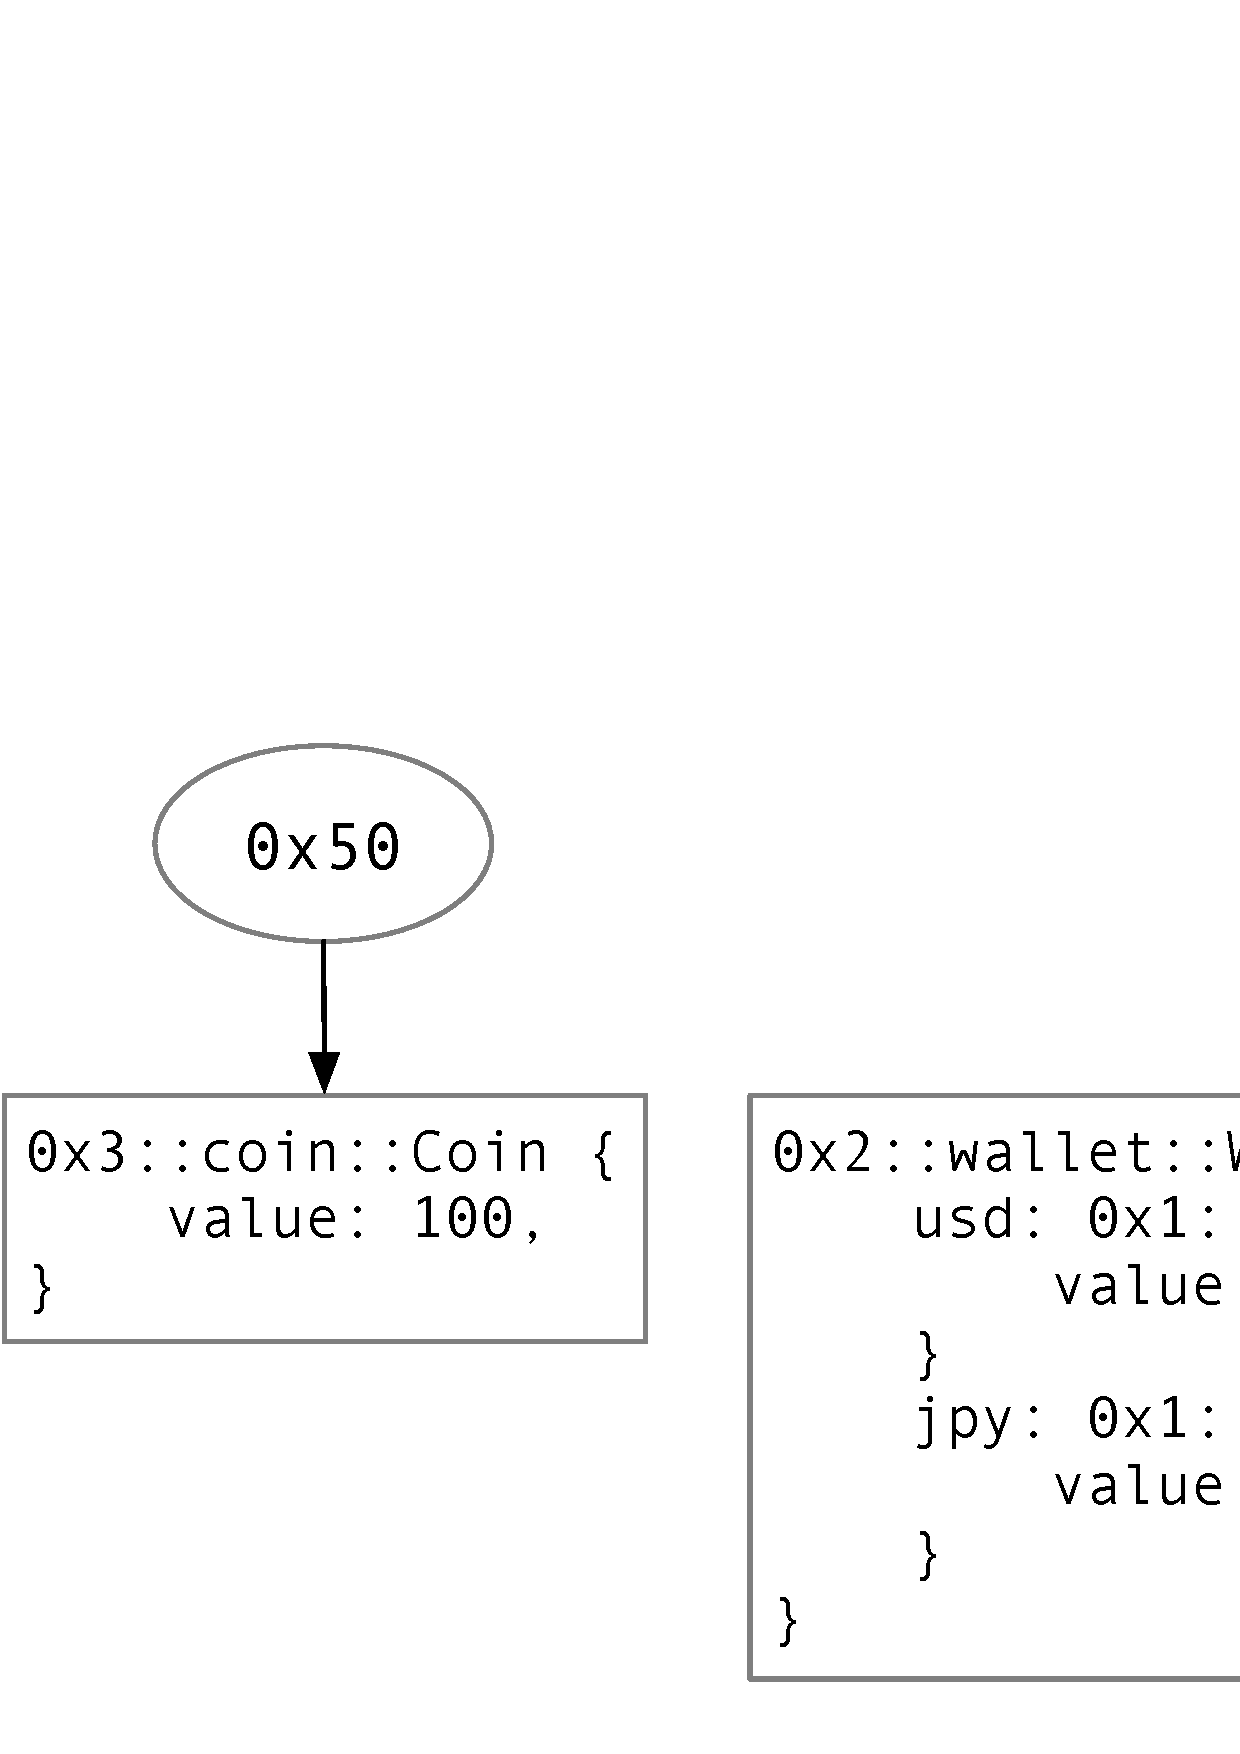
\includegraphics[width=0.95\textwidth]{move_2.png}
\caption{\label{fig:move_data}链上的数据示例。}
\end{figure}

在一个地址下最多具有每个类型的一个顶级值可能起初听起来很有限。但是,这在实践中不是问题,因为程序员可以定义新的数据类型并将原有类型作为其内部字段,从而避免任何限制。图 \ref{fig:move_data} 中的 \mintinline{rust}{Wallet} 结构是如何使用包装器类型的示例。

还应注意,并非所有数据类型都可以存储在链上。为了使数据实例符合顶级值,数据类型必须具有 \mintinline{rust}{key} 能力。同样,嵌套值也需要 \mintinline{rust}{store} 能力。同时具有这两种能力的数据类型通常也被称为 \emph{resources}。


\subsection{账本状态}
\label{sub:ledger_state}

从 Move 虚拟机(Move VM)的角度来看,每个账户都由一组值和键值对数据结构组成。这些数据结构称为 \emph{table entries} ,并以二进制规范序列化格式 (BCS) 存储。这种数据布局可以有效支持不同的编程范式:少量重复数据大量账户,亦或者少数账户大量数据。Move模块的存储方式与帐户数据类似,但在独立的命名空间下。创世账本状态定义了初始账户集及其在区块链初始化时的关联状态。 

在启动时,Aptos 区块链将由一个单一的账本状态表示。然而,随着采用的增加和技术的发展,Aptos 将扩大分片的数量以增加吞吐量(即启用多个分类帐状态)并支持跨分片移动或访问资产的交易。每个账本状态都将维护特定分片的所有链上资产,并为相同的账户模型提供细粒度的键值对数据存储,为存储访问提供近乎固定的成本。


\section{安全的用户体验}
\label{sec:user}

为了覆盖数十亿互联网用户,web3 用户体验必须安全且易于访问。在以下部分中,我们描述了 Aptos 区块链提供的几项创新,旨在实现这一目标。

\subsection{交易可行性保护}
\label{subsec:transaction_replay_protection}

签署一笔交易意味着签署者授权交易由区块链提交和执行。有时,用户可能会无意中签署交易,或者没有充分考虑到他们的交易可能被操纵的所有方式。为了降低这种风险,Aptos 区块链限制了每笔交易的可行性,并保护签名者免受无限有效性的影响。 Aptos 区块链目前提供三种不同的保护—— 发送者的序列号、交易过期时间和指定的链标识符。
\begin{itemize}
\item 一笔交易的序列号对每个发送者的账户最多只能提交一次。因此,发送者可以观察到,如果当前账户的序列号 $\geq$ 交易 $t$ 的序列号,那么要么t已经被提交,要么t将永远不会被提交(因为 $t$ 使用的序列号已经被另一个交易消耗了)。 
 
\item 区块链时间以高精度和频率(通常为亚秒级)推进,详见第 \ref{subsubsec:blockchain_time} 节。如果区块链时间超过了交易 $t$ 的过期时间,那么类似地,要么 $t$ 已经被提交,要么 $t$ 永远不会被提交。
 
\item 每笔交易都有一个指定的链标识符,以防止恶意实体在不同的区块链环境(例如,跨测试网和主网)之间重放交易。
\end{itemize}

\subsection{基于Move的密钥管理}

如第 \ref{sec:accounts} 节所述,Aptos 帐户支持密钥轮换,这是一项重要功能,可帮助降低与私钥泄露、远程攻击以及未来可能破解现有加密算法相关技术突破的风险。此外,Aptos 账户也足够灵活,可以启用新的混合托管模式。在一种这样的模型中,用户可以将轮换帐户私钥的能力委托给一个或多个保管人和其他受信任的实体。然后,Move 模块可以定义一个策略,使这些受信任的实体能够在特定情况下轮换密钥。例如,实体可能由许多受信任方持有的 $k$-out-of-$n$ 多重签名密钥表示,并提供密钥恢复服务以防止用户密钥丢失(例如,目前百分之二十 的比特币被锁定在不可恢复的账户中 \cite{lost_passwords})。 此外,虽然许多钱包支持各种密钥恢复方案,例如将私钥备份到云基础设施、多方计算和社会恢复,但它们通常在没有区块链支持的情况下实施(即脱链)。结果,每个钱包都需要实施自己的密钥管理基础设施,相关操作对用户来说变得不透明。相比之下,在 Aptos 区块链层支持密钥管理功能提供了所有与密钥相关的操作的完全透明性,并使实施具有丰富密钥管理的钱包变得更加简单。

\subsection{签约前的交易透明度}

今天,钱包对其签署的交易几乎没有透明度。因此,用户通常很容易被诱骗签署可能窃取资金并造成毁灭性后果的恶意交易。即使对于需要枚举每笔交易访问的所有链上数据的区块链也是如此。因此,目前几乎没有针对用户的保护措施,使用户容易受到各种各样的攻击。 为了解决这个问题,Aptos 生态系统为交易预执行提供服务:一种预防措施,在签署之前向用户(以人类可读的形式)描述他们的交易结果。将此与已知的先前攻击历史和恶意智能合约相结合将有助于减少欺诈。此外,Aptos 还使钱包能够在执行期间对交易进行限制。违反这些约束将导致交易被中止,以进一步保护用户免受恶意应用程序或社会工程攻击。

\subsection{实用的轻客户端协议}

仅仅依靠 API 提供商的 TLS/SSL 证书在区块链客户端和服务器之间建立信任并不能充分保护客户端。即使存在有效证书,钱包和客户也无法保证所提供数据的真实性和完整性。

\begin{figure}
\centering
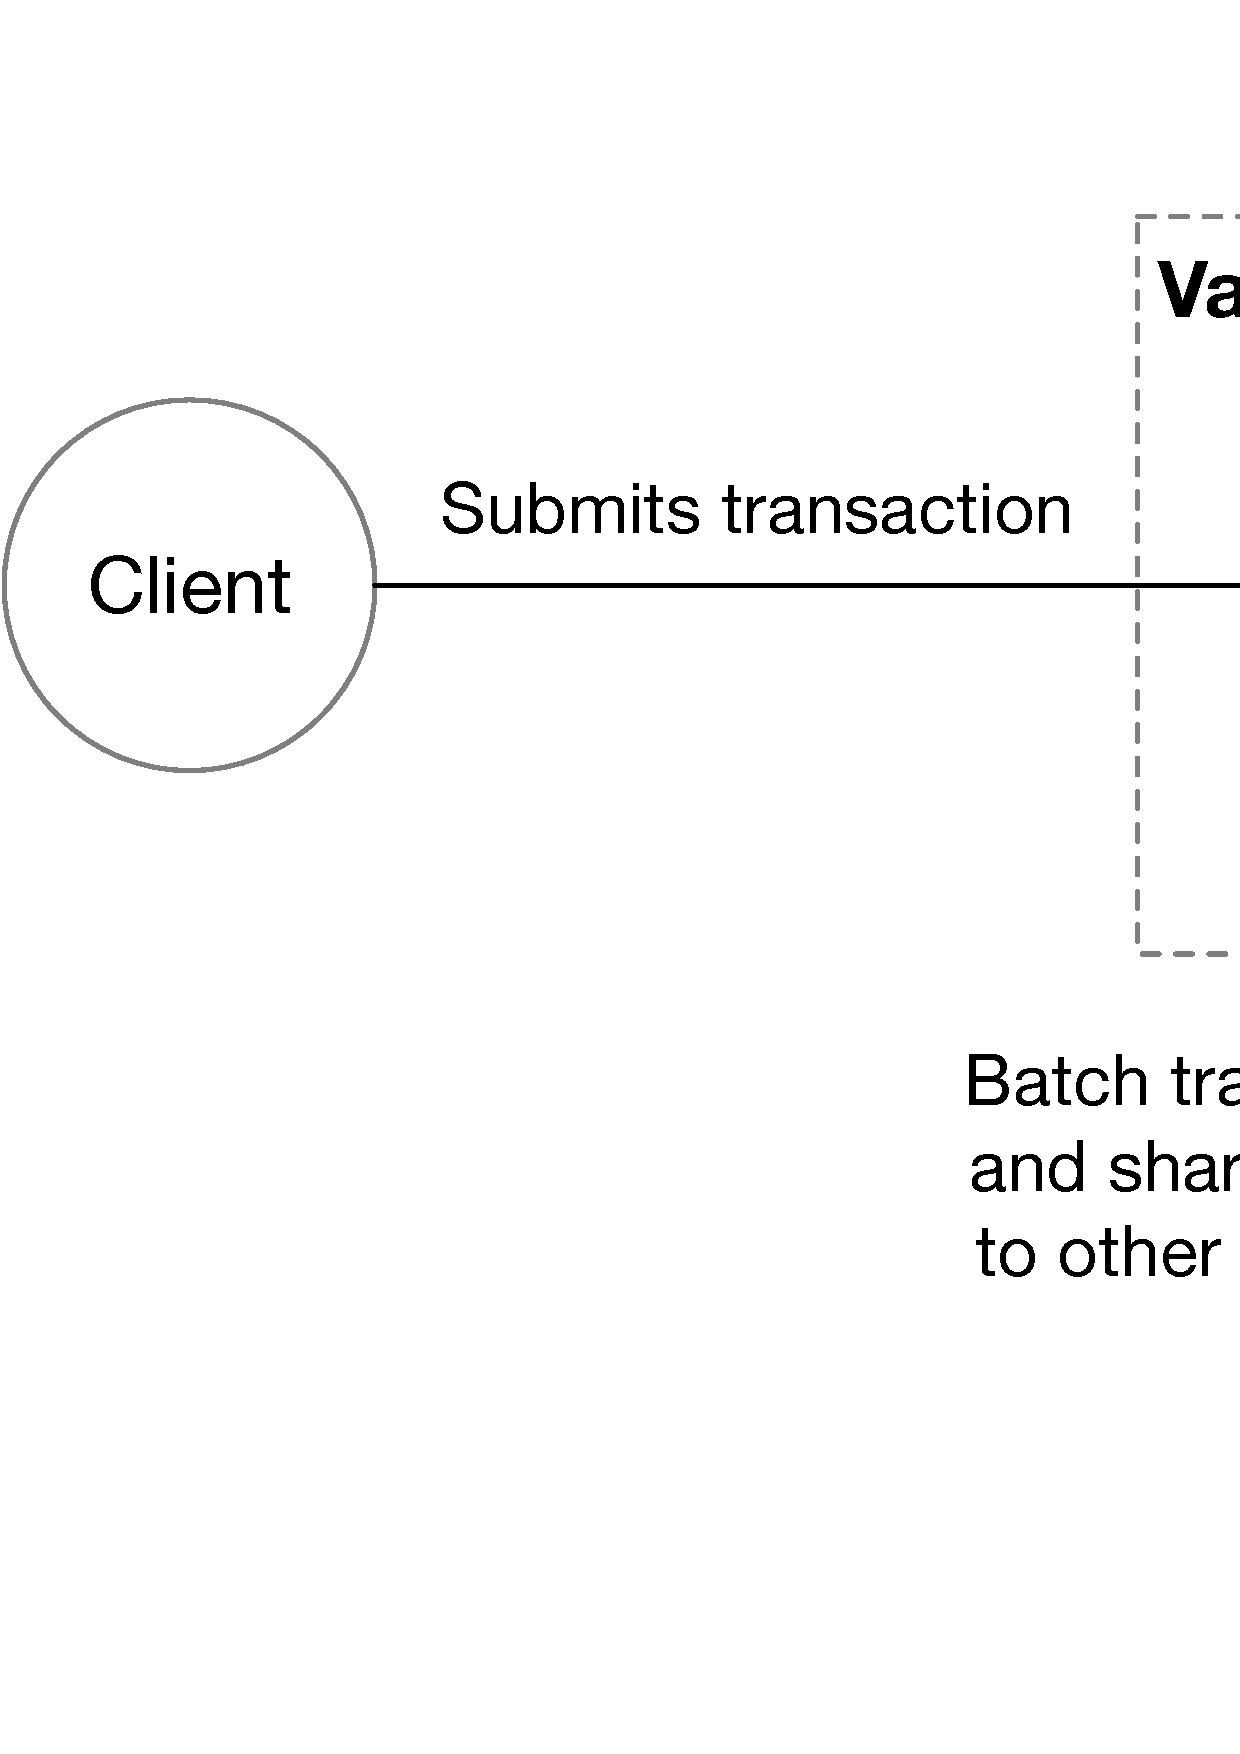
\includegraphics[width=0.95\textwidth]{pipeline.png}
\caption{\label{fig:pipeline}交易处理生命周期。所有阶段都是完全独立的,并且可以单独并行。}
\end{figure}

因此,API 提供商可能会返回不正确或恶意的区块链数据,从而欺骗第三方并执行双花攻击。 为了防止这种情况,Aptos 提供状态证明和轻客户端验证协议,钱包和客户端可以使用这些协议来验证不受信任的第三方服务器提供的数据的有效性。此外,通过利用第 \ref{subsubsec:period_state_certification} 节中基于时间戳的状态证明,轻客户端始终可以确保帐户状态的新鲜度(例如,在几秒钟内)的严格限制,并且只需要跟踪网络配置的变化(\emph{纪元变化})或使用当前受信任的检查点(\emph{关键点})来保持最新状态 \cite{waypoints}。通过结合高频时间戳和廉价的状态证明,Aptos 区块链为客户提供了更高的安全保证。 

此外,Aptos 节点还公开了丰富的高性能存储接口,可以进一步微调以允许订阅针对特定数据和链上帐户的证明。轻客户端可以利用这一点来保留最少的可验证数据,而无需运行完整节点或处理大量事务。


\section{流水线、批处理和并行交易处理}
\label{sec:pipelining_batching}

为了最大限度地提高吞吐量,增加并发性,并降低工程复杂性,Aptos区块链上的交易处理被分为不同的阶段。每个阶段都是完全独立的和单独的可并行化,类似于现代的超标量处理器架构。这不仅提供了显著的性能优势,而且使Aptos区块链能够提供验证者-客户互动的新模式。比如说:

\begin{itemize}
\item 当特定交易已包含在一批持久交易中时,可以通知客户端。 持久且有效的交易极有可能立即提交。

\item 当一批持久化的交易被排序完成时,可以通知客户端。为了减少确定已执行交易结果的延迟,客户端可以选择在本地执行交易,而不是等待验证者节点远程完成执行。
 
\item 客户端可以选择等待验证者节点执行经过验证的交易,并对经过验证的结果执行状态同步(例如,参见第 \ref{sub:state_sync} 节)。
\end{itemize}

Aptos 模块化设计有助于加快开发速度并支持更快的发布周期,因为变更可以针对单个模块,而不是整个单体架构。 同样,模块化设计还提供了将验证者节点扩展到单台机器之外的结构化路径,提供额外的计算、网络和存储资源。 图 \ref{fig:pipeline} 显示了整个事务的生命周期不同的处理阶段.

\subsection{批处理}
批量处理是一个重要的效率优化,是Aptos区块链中每个操作阶段的一部分。在交易传播过程中,交易被每个验证者分组为批次,而在共识过程中,批次被合并为区块。执行、存储和账本认证阶段也分批工作,以提供重新排序、减少操作(例如,重复计算或签名验证)和并行执行的机会。

将交易分组可能会导致少量延迟,例如,在执行分发之前等待 200 毫秒来累积一批交易。 但是,批处理在最长等待时间和最大批量大小方面很容易配置,使去中心化网络能够自动优化延迟和效率。 批处理还允许有效的收费市场对交易进行优先排序,并避免来自过分热心客户的拒绝服务 (DoS) 攻击。


\subsection{持续的交易传播}
\label{continuous_txn_dissemination}

根据Narwhal & Tusk \cite{narwhal_tusk}论文的主要观点,Aptos区块链的交易传播与共识脱钩。验证者不断地相互传输批次的交易,同时利用所有可用的网络资源。由验证者 v 分发的每批交易都被持久化,并将批次摘要的签名发回给 v。在第7.3节中定义,任何 2f+1 个在批次摘要上的加权签名形成一个可用性证明(PoAv)。可用性证明(PoAv)。这样的证明保证了至少有 f+1 个加权的诚实验证者已经存储了该批次,因此所有诚实的验证者都能在执行前检索到它。

无限持续的交易批次可以打开一个DoS攻击的载体,导致验证者节点用完存储并崩溃。为了防止这种情况,每批交易都有一个相关的时间戳。该批交易的时间戳允许在每个验证者节点上进行有效的垃圾回收。此外,一个单独的每个验证者配额机制旨在保护验证者即使在最极端的情况下也不会耗尽空间,例如在潜在的拜占庭攻击下。批次还具有大小限制,在同意保存到稳定存储之前验证这些限制。最后,通过一些优化来消除重复和缓存交易,减少存储成本,并确保与并行执行引擎的高性能集成。

\begin{figure}
\centering
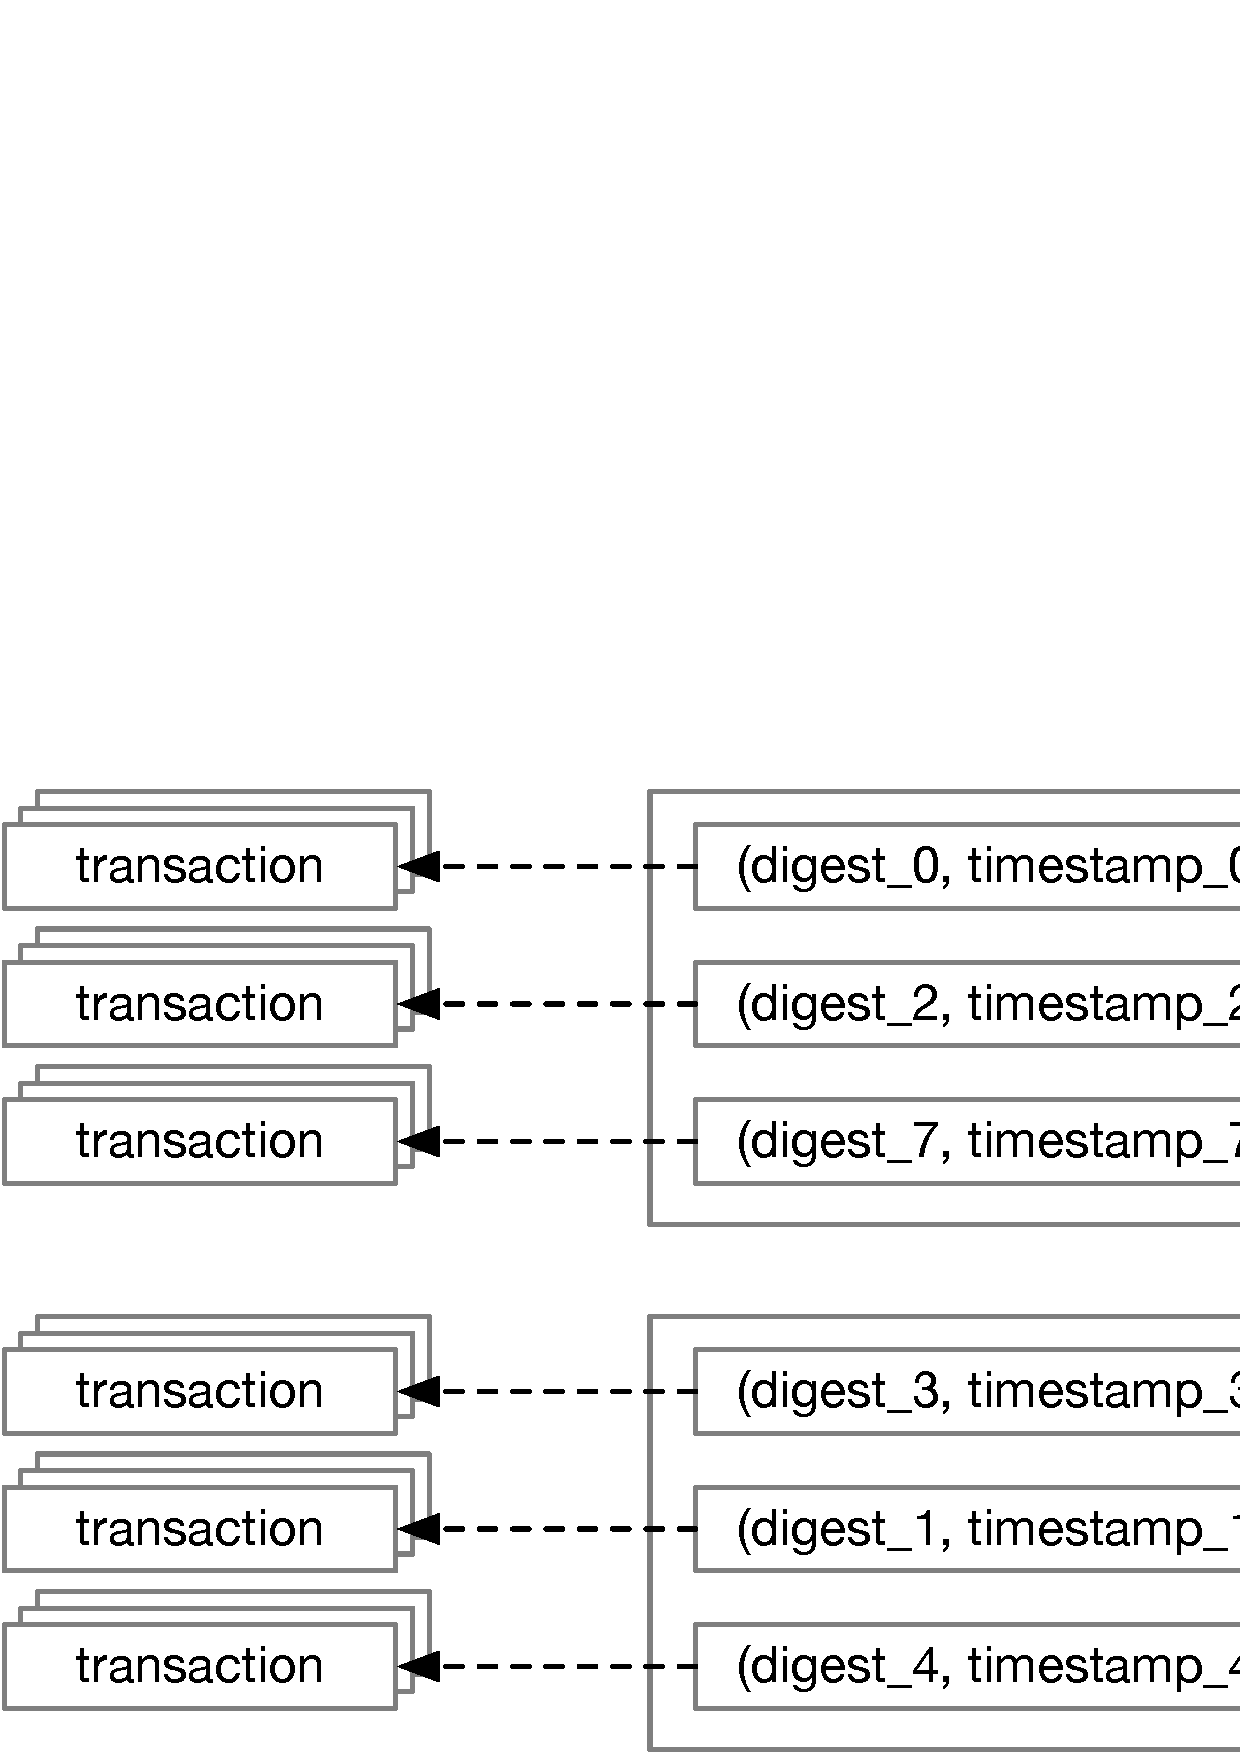
\includegraphics[width=0.95\textwidth]{ordering.png}
\caption{\label{fig:block}区块元数据排序独立于交易传播}
\end{figure}

\subsection{区块源数据排序}
\label{subsec:block_metadata_ordering}

一种常见的误解是共识速度很慢,因此是区块链吞吐量和延迟的主要瓶颈。 Aptos 区块链的关键创新之一是将非协议相关的任务从共识阶段解耦出来,例如交易传播、交易执行/存储和账本认证。通过将交易传播与共识阶段分离,可以在非常低的带宽下进行排序(仅限区块元数据和证明),从而实现交易高吞吐量和最小化延迟。

今天,Aptos 区块链利用了 DiemBFTv4 \cite{diembft_v4} 的最新迭代版本,这是一个乐观的响应式BFT共识协议。普通情况下的共识只需要两次网络往返(全网往返时间通常小于300毫秒),并通过领导者信誉机制 \cite{be_aware} 对有缺陷的验证者进行动态调整。链上领导者信誉机制提升在一个窗口中成功提交区块的验证者,并将没有参与的验证者降级。这种新颖的机制极大地提高了去中心化环境下的性能,相应地提供了适当激励的基础设施,并迅速将失败的验证者对吞吐量和延迟的影响降到最低。

DiemBFTv4  保证了部分同步下的活性,并确保了异步下的安全性,其中总验证者权益 $\geq 3f+1$,最多 $f$ 个权益加权错误验证者。自 2019 年以来,DiemBFTv4 已经在多次迭代中经过了数十个运营商节点和多钱包生态系统的广泛测试。我们还在试验我们最近的研究(例如 Bullshark \cite{bullshark}) 和其他依赖区块历史和相关通信来确定区块元数据排序和最终性的协议。

共识区块和提案时间戳由领导者提出并由其他验证者同意,如图 \ref{fig:block} 所示。请注意,每个共识块仅包含批处理元数据和证明。区块中不需要实际交易,因为 PoAV 确保交易批次在排序后的执行阶段可用(参见第 \ref{continuous_txn_dissemination} 节)。验证者在验证了证明和区块元数据标准(例如,提案时间戳 $\le$ 区块到期时间)后,可以对领导者的提案进行投票。

\subsubsection{区块链时间}
\label{subsubsec:blockchain_time}

Aptos 区块链为每个提案的区块以及该区块内相应的的所有交易采用一个近似的、约定的物理时间戳。此时间戳支持许多重要的用例。例如: 
\begin{itemize}

\item 智能合约中的时间相关逻辑。例如,开发人员希望编码必须在周四中午之前收到拍卖的所有标的。

\item 随着预言机发布链上数据,需要准确且可信的链上时间戳来关联事件并处理来自真实世界数据的延迟。

\item 客户可以辨别他们在区块链方面的最新情况。出于安全原因,为避免过时数据和远程攻击,客户端应有权访问帐户状态更新时间的高精度时间戳。

\item 使用可信时间戳审计区块链提供了与链外事件的强相关性,例如确保合法执行的支出符合预期要求。

\item 交易过期是基于最近提交的时间戳。作为客户端交易的额外保障,客户端可以选择交易的过期时间,如第 6.1 节所述。

\end{itemize}

Aptos 区块链为区块内所有交易的时间戳提供以下保证:

\begin{itemize}
\item 在区块链中时间是单调递增的。也就是说,如果块 $B1 < $ 块 $B2$,则 $B1.Time < B2.Time$。

\item 如果一个交易区块与时间戳 $T$ 达成一致,那么至少有 $f+1$ 个诚实的验证者已经确定 $T$ 是过去的。诚实的验证者只会在自己的时钟 $\ge$ 时间戳 $T$ 时对区块进行投票。参见第 7.2 节。

\item 如果一个交易块具有与时间戳 T$T$ 一致的法定签名,那么诚实的验证者将不会将这样的块提供给其他验证者,直到它自己的时钟 $\ge$ 时间戳 $T$。
\end{itemize}

最近的时间戳在每个提交的区块上更新,并用作该区块中所有交易的时间戳。当网络同步时,每一次网络往返都会提交一个交易区块,并提供快速更新和高度可靠的时钟。如果需要,可以确定交易块内更精细的排序粒度。

\subsection{并行交易执行}
\label{subsec:parallel_transaction_execution}

一旦对共识区块元数据进行排序,任何验证者节点、完整节点或客户端都可以执行交易。至少有 $2f+1$ 个权益加权验证者对提案的批次进行了真正持久的交易。由于交易传播是连续的,额外的诚实验证者将随着时间的推移接收交易批次。如果诚实的验证者节点在到达执行阶段时还没有收到订单批次的交易,它可以从 $2f+1$ 个权益加权验证人下载它们,知道至少有 $f+1$ 个权益加权验证人($\ge$一半的权益加权验证人)权益加权 PoAV 签名者)是诚实的。

任何区块链的一个重要目标是实现尽可能多的并行执行。 Aptos 区块链从数据模型和执行引擎两方面向前推进。

\subsubsection{并行数据模型}

Move 语言数据模型本身支持数据和模块的全局寻址。数据和账户没有重叠冲突的事务可以并行执行。鉴于 Aptos 区块链使用的流水线设计,重新排序一组交易可以减少冲突的数量,从而提高并发性。

即使交易修改了同一组链上值,大部分交易执行过程仍然可以并行化。 Aptos 区块链引入了一个新概念,delta writes,它描述了对账户状态的修改,而不是修改后的账户状态(例如,增加一个整数而不是简单地确定最终值)。所有交易处理都可以并行完成,然后以正确的顺序对冲突值应用增量写入,以确保确定性结果。

随着时间的推移,Aptos 区块链将继续以提高并发性(例如,利用读/写提示)并改善人机工程的方式来增强数据模型,使开发人员更自然地创建、修改和组合链上值。 Move 语言提供了灵活性,可以在语言层面以及特定平台的功能进行这些改进。

\begin{figure}
\centering
\includegraphics[width=0.95\textwidth]{perf.jpg}
\caption{\label{fig:perf}Block-STM(仅组件)比较不同竞争程度时物理核心数变化的基准测试。}
\end{figure}

\subsubsection{并行执行引擎 Block-STM} 

并行执行引擎检测和管理一组有序交易的冲突以及乐观锁并发控制,以在给定特定顺序的情况下实现最大并行度 \cite{block_stm}。

批量交易以乐观方式地并行执行,并在执行后得到验证。不成功的验证会导致重新执行。 Block-STM 使用多版本数据结构来避免写-写冲突。所有对同一位置的写入都与它们的版本一起存储,其中包含它们的交易 ID 和写入交易被乐观锁方式重新执行的次数。当交易 $tx$ 读取一个内存位置时,它从多版本数据结构中获取按预设顺序出现在 $tx$ 之前的最高交易写入该位置的值以及相关版本。

Block-STM 已经集成到 Aptos 区块链中。为了理解 Block-STM 性能的全部潜力,我们将有意义的点对点 Move 交易(即每个交易 8 次读取和 5 次写入)作为隔离的、仅执行的(不是端到端的)进行了实验) 使用内存数据库进行基准测试。在图 \ref{fig:perf} 中,我们展示了我们的 Block-STM 执行结果。每个区块包含 10k 笔交易,账户数量决定了冲突和争用的程度。在低争用情况下,Block-STM 在 32 个线程的顺序执行中实现了 16 倍的加速,而在高争用情况下,Block-STM 实现了超过 8 倍的加速。与区块链空间中的其他并行执行引擎不同,Block-STM 能够动态且透明地(无需用户提示)从任何工作负载中提取固有的并行性。与需要预先了解要读取或写入的数据位置的并行执行环境相比,BlockSTM 可以同时支持更复杂的事务。此属性导致更少但更高效的事务,降低成本,并为用户提供更低的延迟。更重要的是,将原子事务拆分为多个较小的事务会破坏具有复杂状态结果的单个事务的全有或全无语义。在 Block-STM 中将富有表现力的事务语义与并行执行结合起来,使开发人员能够两全其美。

请注意,区块元数据排序步骤不排除在并行执行阶段重新排序交易。交易可以跨一个或多个区块重新排序,以优化并行执行的并发性。唯一的要求是所有诚实验证者节点的重新排序必须是确定性的。优化并行执行以及在重新排序中添加随机化可以提高性能,并可能阻止利用最大可提取价值 (MEV) 技术唯利是图的验证者对交易进行重新排序。 在这个流水线设计中,也可以加入 "先订后揭 "的抗MEV策略。 

Block-STM 和交易重排是增加执行并行性的补充技术。它们可以与交易读/写访问提示结合使用,以实现额外的并发性。

\subsection{批量存储}

并行执行阶段的结果是一个组中所有事务的写入集。这些写入集可以存储在内存中以获得最大的执行速度,然后用作下一个区块或要执行的区块集的缓存。任何重叠写入只需要写入稳定存储一次。如果验证者在存储内存写入集之前失败,它可以简单地从区块元数据排序阶段恢复并行执行。将写入集的批量存储与并行执行步骤分离,确保并行执行能够高效运行。总之,批处理写入集减少了存储操作的数量,并利用了更高效、更大的 I/O 操作。

可以为每台机器手动配置为写入集缓存保留的内存量,并提供自然的反压(back-pressure)机制。如果需要针对特定 I/O 和内存环境进行调整,批处理的粒度可以不同于并行执行块的粒度。

\subsection{账本(Ledger)认证}

在流水线这一点上,每个单独的验证者都已经计算了已提交交易区块的新状态。然而,为了有效支持经过验证的轻客户端和状态同步,Aptos 区块链对账本历史和账本状态实施了账本认证。 Aptos 区块链的一个关键区别是账本认证不在交易处理的关键路径上,如果需要,甚至可以完全带外(out-of-band)运行。

\subsubsection{账本(Ledger)历史认证}
\label{subsubsec:ledger_history_certification}

验证者节点将交易连同它们的执行输出一起附加到全局认证的账本数据结构中。交易输出的一部分是状态写入集,包括对 Move  可访问的全局状态所做的更改。该数据结构的短验证者是对账本历史的绑定承诺,其中包括新执行的一批交易。与交易执行类似,这种数据结构的生成是确定性的。

每个验证者节点将认验器签名到生成的数据库的新版本。验证者节点彼此共享他们最近的一组签名短身份认证器,集体汇总法定签名短认证器,并且还相互分享最近的法定签名短认证器。

根据 BTF 协议的属性,使用这种集体签名,客户可以相信数据库版本代表了完整、有效和不可逆的账本历史。客户端可以查询任何验证者节点(或数据库的任何第三方副本,例如完整节点)以读取数据库值并使用认证器和所需数据的证明来验证结果。

\subsubsection{定期状态认证}
\label{subsubsec:period_state_certification}

Move 语言可访问的整个全局状态可以在历史的任何时间点汇总到一个简短的认证器,类似于账本历史的摘要。由于全局状态的随机访问性质(与仅追加的账本历史不同),维护此认证的成本很高。然而,在大批量更新数据结构时,我们可以并行计算更新,并且还可以利用每个单独状态值更改时必须更新的部分之间的任何重叠。 Aptos 区块链有意使用定期验证全局状态以减少重复的共享更新。

在确定性和配置的时间间隔内,网络发出状态检查点事务,其中包括全局状态认证器作为其输出的一部分。这样的版本被称为状态检查点。两个检查点之间的差距越大,每笔交易更新经过状态验证的数据结构的摊销成本就越低。

有了状态检查点,可以以一种无需信任的方式从中读取任何状态值,而无需存储所有全局状态。这种能力对于增量状态同步、跨验证者节点的分片存储、无状态验证者节点和存储受限的轻客户端等应用程序非常有用。

但是,由于状态检查点是周期性的,因此要获得特定版本的账本状态的证明,需要对丢失的状态交替执行额外的交易,或者从经过认证的账本历史中获得包含它们的证明。

状态检查点与账本历史中的特定交易版本相关联,因此与第 7 节中提到的与交易批次相关的时间戳绑定。有了时间戳,轻型客户可以了解被证明的状态值的时间性。如果没有时间戳,轻客户端证明只能确保以前的状态的有效性,而这个状态可能是过去很久以后的事情,这几乎不能保证其相关性。此外,状态证明的时间戳对于跟踪历史访问和审计目的是必要的,例如计算代币储备中的平均每小时余额。

状态检查点可以基于先前的状态检查点和之后的交易输出中的状态变化来推导出来。因此,将状态检查点持久化到稳定存储并不需要处于事务处理的关键路径上。此外,在持久化状态检查点时也存在有益的批处理效果。在内存中缓存最近的状态检查点(或者更确切地说是它们之间的增量)并仅将周期性状态检查点转储到稳定存储中可以大大减少存储带宽的消耗。选择持久化检查点的方式不会影响经过认证数据结构的计算。因此,这是每个节点的选择:节点运营商可以在内存容量和存储带宽之间进行适当的权衡。


\section{状态同步}
\label{sub:state_sync}

Aptos 区块链旨在为生态系统中的所有参与者提供一个高吞吐量、低延迟的系统。因此,区块链必须提供一个有效的状态同步协议来传播、验证和持久化区块链数据到轻客户端、全节点和验证者 \cite{evolution_state_sync}。此外,考虑到不同的用户和用例,同步协议还必须能够容忍网络内的资源限制和异构性。例如,它必须允许归档完整节点验证和保存整个区块链历史和状态,同时还允许轻客户端有效地跟踪 Aptos 区块链状态的一小部分。

为了实现这一特性,Aptos 区块链利用验证者节点、完整节点和其他复制器提供的经过验证的账本历史记录和经过验证的状态证明(参见第 \ref{subsubsec:ledger_history_certification} 节)来提供灵活且可配置的同步协议。具体来说,网络中的参与者可以选择不同的同步策略来优化他们的用例和需求。

例如,在全节点的情况下,Aptos 允许多种同步策略,包括处理自时间开始以来的所有交易或完全跳过区块链历史并使用关键点仅同步最新区块链状态的能力。在轻客户端的情况下,策略包括同步部分区块链状态,例如特定账户或数据值,并启用已验证状态读取,例如,已验证帐户余额获取。在所有情况下,Aptos允许参与者配置获取、处理和保留数据的数量和时间。留。

通过采用灵活且可配置的状态同步方法,Aptos 可以适应各种客户需求,并在未来继续提供新的、更高效的同步策略。

\section{社区所有权}
\label{sec:community_ownership}

Aptos 区块链将由一个多元化的社区拥有、运营和管理,原生 Aptos 代币将用于交易和网络费用、协议升级和链上/链下流程的治理投票,以及通过权益证明模型来保护区块链。Aptos token经济学的完整说明将在未来的出版物中发布。


\subsection{交易和网络费用}
\label{subsec:network_fees}

所有Aptos的交易都有gas单价(用Aptos token标价),这使得验证者可以优先处理网络中价值最高的交易。而且,在流水线模型的每个阶段,都有多个机会放弃低价值的交易(允许区块链在达到系统容量时也能有效地运行)。随着时间的推移,将部署网络费用,以确保使用Aptos区块链的成本与实际部署的硬件、维护和节点运维成本相当。此外,开发者将有机会在设计应用程序的时候可以依据算力、存储和网络之间不同的成本进行权衡。


\subsection{网络治理}
\label{subsec:network_governance}

Aptos区块链上的每一个重大特性的变更及改进都将经历这几个阶段:提案、实现、测试和部署。这样的流程让有关人士及利益相关者能够有机会去提供反馈、共享问题和提出建议,最后一个阶段,即部署,通常会有两个步骤。首先会将带有新功能的软件版本部署到每个节点,其次启用这个功能将,例如,通过特性标志或链上(on-chain)配置变量。

节点运维人员的每个软件部署必须是向后兼容的,以确保新的软件与支持的版本可以互操作。部署一个新的软件版本的过程的过程可能会持续多天,以顾全不同时区的运维和任何外部问题。 一旦升级了足够数量的节点,新功能的启用就可以由一个同步点触发,比如一个约定的区块高度或纪元(epoch)切换。在紧急条件下(例如,当停机时间不可避免时),可以通过节点运维人员手动和强制改变来启用。在最坏的情况下,对网络硬分叉。

与其他区块链相比,Aptos区块链对其配置进行链上编码。每个验证者都能同步区块链的当前状态,并根据当前的区块链状态自动选择正确的配置(例如,共识协议和Aptos框架版本)。由于这一功能,Aptos区块链的升级是无缝和即时的。

为了给启用过程提供灵活性和可配置性,Aptos区块链将支持链上治理,代币持有者可以根据他们持有的代币权重进行投票。链上投票协议是公开的、可验证的,并且可以是即时的。链上治理还可以支持在没有软件部署的情况下实现非二元结果。 例如,链上leader选举协议参数可以通过链上治理进行修改,而预先知道的同步点将不用处理动态修改,因为所有更改都必须提前知道。

随着时间的推移,链上治理可以部署在整个升级管理过程中。举个例子:

\begin{enumerate}
\item 代币持有人在链上投票决定过渡到新的抗量子计算签名方案
\item 开发人员实施和验证新的签名方案,并创建一个新的软件版本
\item 验证者升级他们的软件到新的版本
\item 代币持有人在链上就启用一个新的签名方案进行投票,链上的配置被更新,变更生效。
\end{enumerate}

作为一个开源项目,Aptos区块链将依赖于强大的社区反馈,并使用链上治理来管理适当的流程。在某些情况下,可能仍然需要链外升级,但随着时间的推移,这种情况将尽量最小化。


\subsection{权益证明共识}
要参与Aptos区块链上的交易验证,验证者必须拥有最低要求的Aptos代币抵押。在交易传播过程中,抵押金额成比例地影响$2f+1$抵押金额 \emph{PoAv} ,以及在区块元数据排序过程中的投票权重和leader选举。验证者决定他们自己和他们各自的投保人之间的奖励分配。质押者可以选择任意数量的验证者来质押他们的代币,以获得预先约定的奖励分配。在每个纪元结束时,验证者和他们各自的抵押者将通过相关的链上Move模块收到他们的奖励。
任何拥有足够抵押的验证者运营商都可以自由加入Aptos区块链。所有的参数包括所需的最低收益,都可以由第 \ref{subsec:network_governance} 节中描述的链上启用程序来设置。


\section{性能}
\label{sec:performance}

如第 \ref{sec:pipelining_batching} 节所述,Aptos区块链能够通过其并行、批量优化和模块化的交易流水线处理实现最佳吞吐量和硬件效率。额外的性能举措,如共识升级、delta写入、交易提示和关键路径缓存,将继续增加吞吐量并随着时间推移提高效率。

今天,区块链的吞吐量通常以每秒交易量来衡量。然而,鉴于各种交易和基础设施的成本和复杂性差异很大,这样的方法比较体系是不精确的。交易延迟也同样存在缺陷,因为在不同的实验中,提交到最后的起点和终点是不同的。

此外,有些系统需要对交易的输入和输出有前置知识,并强制将逻辑交易分割成较小的、不太复杂的交易。 分割交易会导致糟糕的用户体验,并人为地影响延迟和吞吐量,而不考虑开发者想要完成的任务。与此相反,Aptos的方法是让开发者能够不受限制地自由构建,并根据实际使用情况测量吞吐量和延迟。自由构建,并根据真实世界的用例而不是合并交易来测量吞吐量和延迟。

Aptos区块链将继续优化单个验证者的性能,以及试验将更多验证者添加到网络的扩展技术。这两个方向都有明显的取舍。任何具有并行执行能力的区块链都可以通过更强大的硬件或将每个验证者构造成一个单独的机器集群支持额外的并发。然而,全局验证者的数量是有实际限制的,它与验证者运维的成本和复杂性是相称的。serverless数据库在云服务中的兴起和流行,体现了很少有实体能够有效地部署和维护这些类型的复杂分布式系统。


\subsection{同质化的状态分片}
最初,Aptos区块链将以一个单一的账本状态推出。随着时间的推移,Aptos网络将采取一种独特的方法来实现横向可扩展性,同时仍然保持去中心化。这将通过多个分片账本状态来实现,每个分片都提供同质化的API和分片是作为一流的概念。Aptos代币将用于所有分片上的交易费、押金和治理。

数据可以通过同构桥(homogeneous bridge)在分片之间传输。用户和开发者可以根据自己的需要选择自己的分片方案。例如,开发人员可以提出一个新的分片,或在现有的分片内对用户进行集群,以实现分片内的高连接。此外,分片可能有不同的系统特性。 一个分片可能是对固态硬盘(SSD)计算优化的,而另一个分片可能是为大型硬盘优化的,计算特性较低。通过在不同的分片之间提供硬件灵活性,开发者可以利用适当的系统特性来满足他们的应用。

总之,同质状态分片提供了水平吞吐量扩展的潜力,允许开发人员在分片中使用单一的通用状态进行编程,并使钱包能够为其用户轻松纳入分片数据。这提供了显著的性能优势,以及一个统一的Move智能合约平台的简洁性。

\nocite{*}
\bibliographystyle{IEEEtran}
\small{
\bibliography{bibtex}
}

\end{document}